% 1960 年全国卷第 6 题：底面为正方形的四棱锥 P-ABCD。
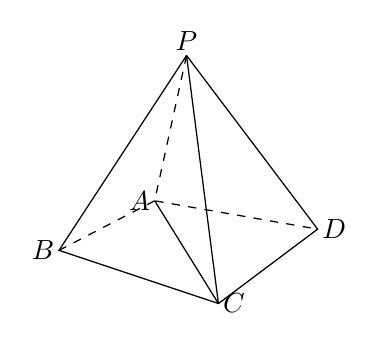
\begin{tikzpicture}[scale=0.9, line width=0.45pt,
  every node/.style={inner sep=1.5pt}]
  \coordinate (P) at (-0.2,2.7);
  \coordinate (A) at (-0.65,0.65);
  \coordinate (B) at (-2.0,-0.05);
  \coordinate (C) at (0.25,-0.8);
  \coordinate (D) at (1.65,0.25);
  \draw (P)--(B)--(C)--(D)--(P);
  \draw (P)--(C);
  \draw[dashed] (P)--(A)--(D);
  \draw[dashed] (A)--(B);
  \draw (A)--(C);
  \node[anchor=south] at (P) {$P$};
  \node[anchor=east] at (A) {$A$};
  \node[anchor=east] at (B) {$B$};
  \node[anchor=west] at (C) {$C$};
  \node[anchor=west] at (D) {$D$};
\end{tikzpicture}
